% The first argument is the script location/filename and the second is a caption for the listing
\subsection{Meep}
\label{ss:c1_meep}

Meep es un software desarrollado en el Massachusetts Institute of Technology - MIT
que implementa el método FDTD. 
Su nombre es un acrónimo que proviene de las iniciales de 
“MIT Electromagnetic Equation Propagation” y cuenta con las siguientes características:

\begin{itemize}
\item Simulación 1D, 2D, 3D
\item Soporte MPI
\item Fronteras Absorción  PML 
\item Scripts  en Scheme (*.ctl)
\item Scripts en C++
\item Análisis de flujos, frec, energía ...
\item Licencia GNU/GPL
\end{itemize} 

\subsubsection{Filtro Notch}

El código está dividido en 5 secciones en cada una de las cuales se define: 
\begin{enumerate}
\item Parámetros de la simulación.
\item Materiales y geometría a simular.
\item Fuente de onda electromagnética.
\item Puntos de medición de flujo de energía.
\item Tiempos y salidas de la simulación.
\end{enumerate} 

\subsubsection{Parámetros}
\zcodectl{"sources/c1_meep_s1.ctl"}{Parámetros Filtro Notch.} 
En esta sección de código (Ver Listing \ref{"sources/c1_meep_s1.ctl"}) 
se especifican los parámetros necesarios para la ejecución de los programas. 
Se usaron 2 tipos diferentes de instrucciones: $define$ y $define-param$. 
La primera instrucción, de la forma $(define <variable> <expresion>)$, es nativa de Scheme y permite 
ejecutar una expresión dada por medio de una variable. 

Por el contrario, $define-param$, está definida en una librería de extensión llamada LibCtl y permite que la 
asociación de la variable a la expresión sea modificada desde la línea de comandos desde la que se invoca el 
programa permitiendo tener un control flexible para las simulaciones. 

Los parámetros usados en la simulación del filtro son:(Ver Tabla \ref{tb:meep_params})

\begin{table}
\centering
\begin{tabular}{| l | l | c | }
\hline
Parámetro & Descripción & Valor x Defecto \\
\hline
$w$ &	Ancho de la guía de onda &  4 nm \\
$r$ &	Radio interno del anillo resonador &	2.9 $\mu$m \\
$gap$ &	Espacio entre la guía de onda y el anillo & 1 nm \\
$dpml$ &    Ancho de la capa PML &  2  $\mu$m \\
$wavecen$ & Ancho de banda central de la fuente &   1550 nm \\
$waveid$ &  Ancho del pulso de la fuente &  50 nm \\
$freqcen$ & Frecuencia central de la fuente &	$\frac{1}{wavecen}$ \\
$freq_width$ &	Ancho del pulso de la fuente (en frecuencia) &	$\frac{1}{wavecen-waveid} - \frac{1}{wavecen+waveid}$ \\
\hline
\end{tabular}
\caption{Parámetros}
\label{tb:meep_params}
\end{table}


\subsubsection{Materiales y Geometría}

En esta sección se emplearon algunos de los parámetros definidos en
la tabla \ref{tb:meep_params} para construir la geometría del filtro como se ve en
la figura \ref{fig:notch_geometry}.

Como se aconseja en \cite{MassachusettsInstituteofTechnology} 
el tamaño del látice a simular se calcula 
de forma dinámica a partir de los parámetros del radio, ancho de la guía de onda, 
espacio de holgura y el borde PML (Ver Listing \ref{"sources/c1_meep_s2.ctl"}). 
%TODO Referencia Tutorial MEEP%

\zcodectl{"sources/c1_meep_s2.ctl"}{Geometría y Materiales Filtro Notch.} 
Silicon Photonics utiliza, como su nombre lo indica, silicio como medio para la propagación de ondas electromagnéticas en el espectro C-Band . 
Por lo tanto, para la longitud de onda de 1500 nm, el índice de refracción del silicio corresponde a 3.4765 \cite{bass2009handbook}. 
Adicionalmente, al ser una simulación en 2D, el material que rodea la guía recta y circular es el aire cuyo índice de refracción es 1. 
La base de dioxido de silicio SiO2 sobre la cual está montada la guía, sólo se tomó en cuenta para la simulación 3D (sección \ref{ss:lumerical}).

%TODO Preguntarle a jose: http://ab-initio.mit.edu/wiki/index.php/Meep_Tutorial 
%Thus, 0.15 corresponds to a vacuum wavelength of about 1 / 0.15 = 6.67, or a wavelength of about 2 in the  material—thus, our waveguide is half a wavelength wide, which should hopefully make it single-mode. (In fact, the cutoff for single-mode behavior in this waveguide is analytically solvable, and corresponds to a frequency of 1/2√11 or roughly 0.15076.)

La guía de onda se especifica como un rectángulo de Si, mientras que la estructura del anillo se construye a partir de la superposición de un cilindro externo de silicio y un cilindro interno de aire. 
Las dos estructuras están separadas en su punto más cercano por una distancia 
definida por el parámetro $gap = 100nm$.

Finalmente, se indicó una resolución de 

\begin{figure}[h!]
\caption{Geometría Filtro Notch.}
\centering
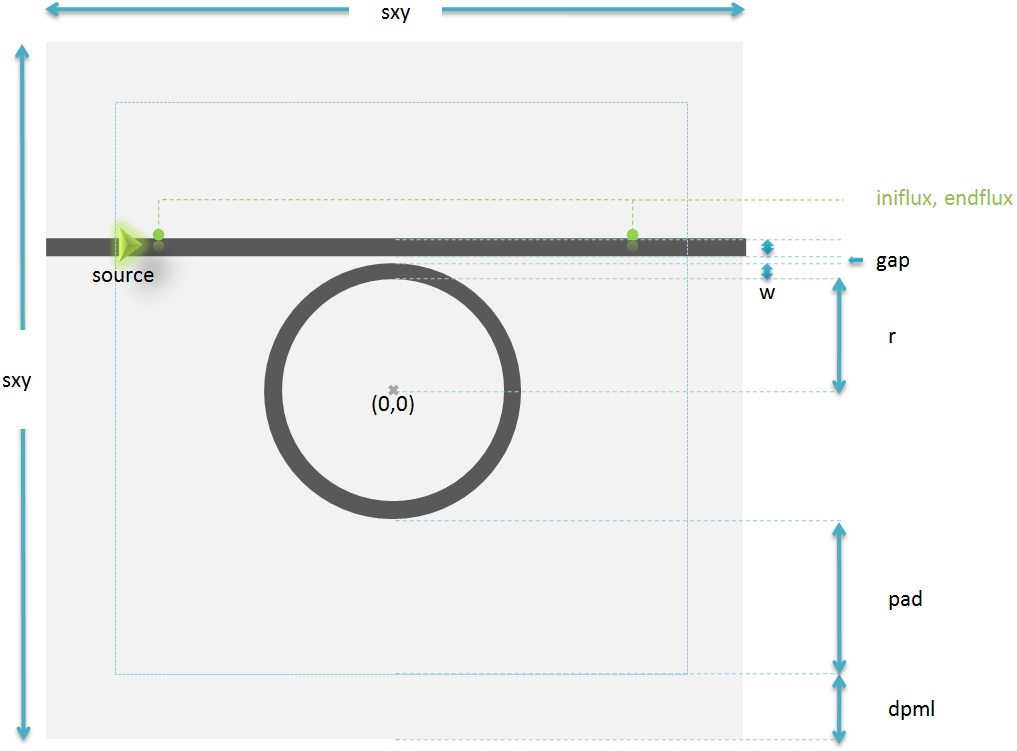
\includegraphics[width=1.0\textwidth,natwidth=892,natheight=663]{figs/notch_v2.jpg}
\label{fig:notch_geometry}
\end{figure}

\subsubsection{Fuente de Onda Electromagnética} 

\subsubsection{Resultados}

\begin{figure}[h!]
\caption{Transmitancia Filtro Notch}
\centering
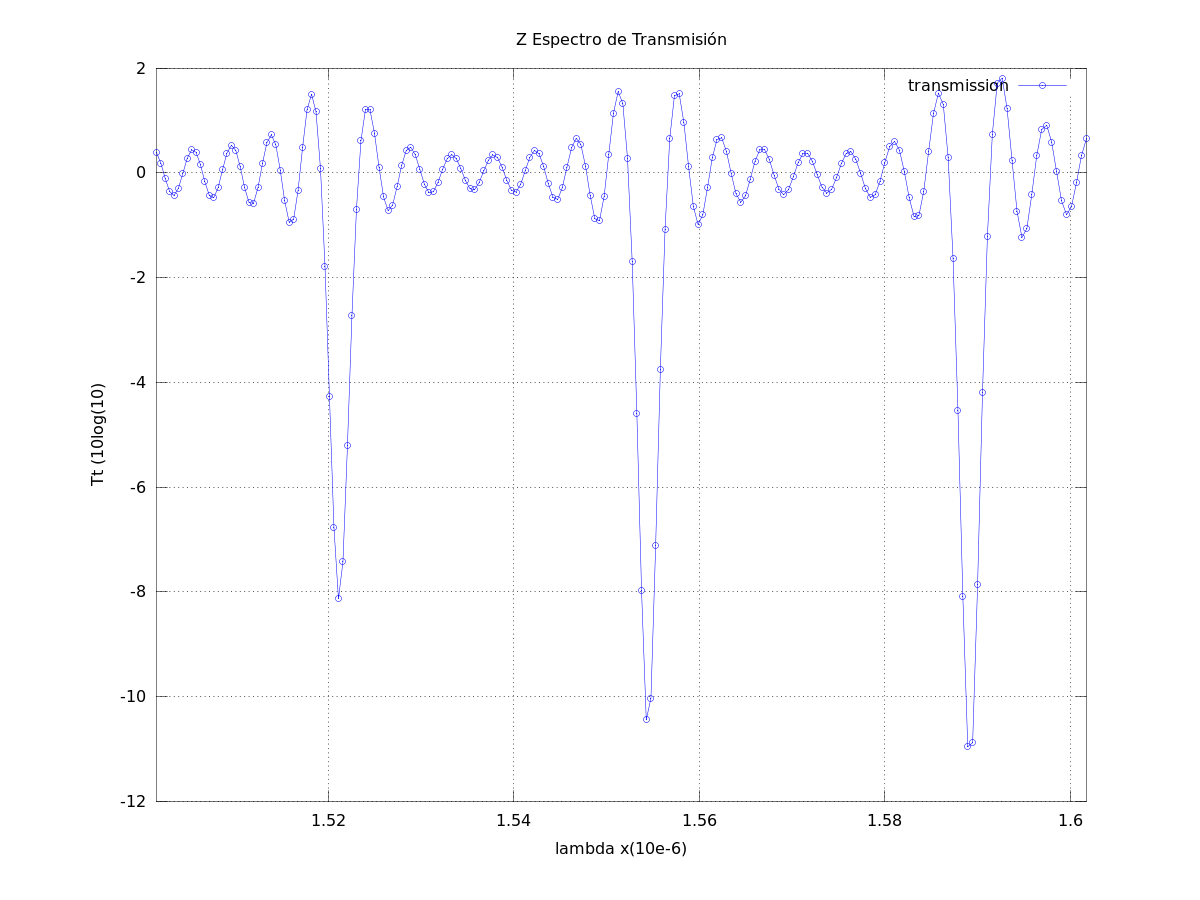
\includegraphics[width=1.0\textwidth,natwidth=1200,natheight=900]{figs/gausrc_flux_mod-graph_res80.png}
\label{fig:meep_res_n}
\end{figure}

